\section{Analysis Categories}
\label{sec:category}

\subsection{Definition of categories and binning}
\label{subsec:cat-motivation}

This analysis, as well as previous iterations, used the invariant mass of the HH system (\mhh) as the discriminating variable for the fit \cite{EXOT-2016-31,ATLAS-CONF-2021-035,HDBS-2018-18-witherratum}.\footnote{The previous ggF searches actually used corrected \mhh to scale the 4-vectors of the HCs to match the Higgs mass of 125 GeV. This modified definition of \mhh helped constrain the widths of the signal peaks in resonant searches.} A multi-variate algorithm (MVA) such as a BDT or NN would provide additional discrimination power; however, given our fully data driven background estimate, using a MVA may affect our ability to validate the modelling of the correlations between the input variables.
%As an example of this, the CMS non-resonant 4b analysis iterations have used a BDT for signal verses background discrimination, but see $2 \sigma$ tensions between the observed and expected limits due to the difficulty of accurately modeling the highest purity BDT bins \cite{CMS-HIG-17-017,CMS-PAS-HIG-20-005}. 
%Although a signal verses background BDT was investigated for the ggF analysis as well and improved the expected limits, 
As a compromise, a number of discriminating variables are used to define extra categories of $S / \sqrt{B}$ purity instead.

As alluded to in \Sect{\ref{sec:selection}}, \deta is a powerful discriminating variable for both the ggF and VBF analyses, and is used as a categorization variable for both these channels (see \Fig{\ref{fig:ggF-4b-deta-xhh-SR}} and \Fig{\ref{fig:vbf-detahh}}).
Specifics of the differences between the ggF and VBF categorization will be described in \Sect{\ref{subsubsec:ggF-cats}} and \Sect{\ref{subsubsec:VBF-cats}}, respectively, along with a visualization of \mhh distributions in each category.
A crucial step in implementing a categorization is ensuring the background within each category is well-modelled. In \Sect{\ref{sec:cats-CR1-validation}} are histograms of the background model in the CR1 training region. Good closure is observed.

Further tests of this categorization and validation of the background estimate are given in \Sect{\ref{sec:bkgvalidation}}.

Since the \mhh distribution is steeply falling, variable width histogram binning -- with narrower bins at low \mhh and wider bins at high \mhh\ -- is used in each of the categories. This allows the analysis to take advantage of the high \mhh events by having reasonable statistical uncertainties within these bins.

A logarithmic binning scheme was chosen. After defining the lowest bin edge, the second bin edge is set at (100 + X\%) $\times$ the lowest bin edge, where X is the specified percentage parameter. Then, the third bin edge is set at (100 + X\%) $\times$ the second bin edge. Bins of increasing width are added in this way until a upper threshold is surpassed. So, going from the lowest bin edge to the highest, the distance to a bin edge is a constant percentage increase on the previous bin edge. Note, the upper threshold is not the last bin edge. An algorithm is used to calculate the bin edges, and once it calculates a bin edge above this upper threshold, it adds it and stops.

Different logarithmic binning parameters are used for the ggF and VBF channels. These are shown in Table~\ref{tab:binning-hyperparameters}. These parameters were optimised to keep the relative error on the quadrature sum of the bootstrap and 2b Poisson components of the background model less than 30\%, whilst not making the bins so wide as to lose important shape information. This 30\% limit was chosen as it corresponds to the relative statistical error on 10 events, the rough threshold at which the asymptotic formulae used in limit setting are valid \cite{Cowan:2010js}. The plots demonstrating that the binning parameters satisfied this are shown in \App{\ref{app:binning}}.

For the ggF channel, the same binning was used across categories (see \Sect{\ref{subsubsec:ggF-cats}}), as the \mhh distributions differ little (as can be seen in \Fig{\ref{fig:ggF-4b-disc-log}} or \Fig{\ref{fig:ggF-4b-disc}}). For VBF, the length of the tails of the \mhh distribution in the two \deta categories differs greatly (\Fig{\ref{fig:vbf-mhh-same}}). As such, different parameters were used. The ggF histograms use bin boundaries rounded to the nearest 1~GeV and the VBF histograms use bin boundaries rounded to the nearest 5~GeV. For ggF, the underflow is included in the lowest bin and overflow is included in the highest bin. Whilst, for VBF, the underflow and overflows are defined as additional bins taking all events below and above the nominal binning.

\begin{table}[tbh]
\begin{center}
	\caption{Parameters used in the \mhh logarithmic binning algorithm. \textit{Min} refers to the starting lowest bin edge and \textit{Max} refers to the upper threshold after which the algorithm adds the last bin edge and stops.}
	\label{tab:binning-hyperparameters}
\begin{tabular}{| c | c | c | c | c |}
 \hline
 {} & Min [GeV] & Max [GeV] & Percentage [\%] & Rounded to Nearest [GeV] \\ 
 \hline\hline
 ggF All Categories & 280 & 950 & 9  & 1 \\ 
 \hline
 VBF low \deta & 280 & 890 & 10 & 5\\
 \hline
 VBF high \deta & 290 & 1470 & 9 & 5\\
 \hline
\end{tabular}
\end{center}
\end{table}

Another method for choosing the binning in \mhh was tested. This was based on an algorithm that systematically merged bins until the statistical uncertainty was under 30\%. This more flexible method resulted in more complicated binning scheme but very close significance and limits, giving us confidence that our simplified category choices are close to optimal.

\subsubsection{ggF categories}
\label{subsubsec:ggF-cats}

The ggF channels are categorized in two variables -- \deta and \Xhh. These variables are already cut on in the ggF channel -- \deta < 1.5 for the QCD background rejection and \Xhh < 1.6 for the SR definition.
The distributions of these two variables of background prediction in the SR are shown in \Fig{\ref{fig:ggF-4b-deta-xhh-SR}}, with overlaid the signal shapes. 
Since the background \deta distribution is flat, three equally spaced \deta bins were chosen between 0 and 1.5. Additionally, two \Xhh bins were defined, with the boundary of 0.95 chosen to equally split the correctly paired signal events. This boundary choice also optimized $S / \sqrt{B}$ significance for the SM NR ggF signal.

\begin{figure}[ht]
	\centering
	\subfloat[All year merged: 4b ggF \deta]{ 
	    	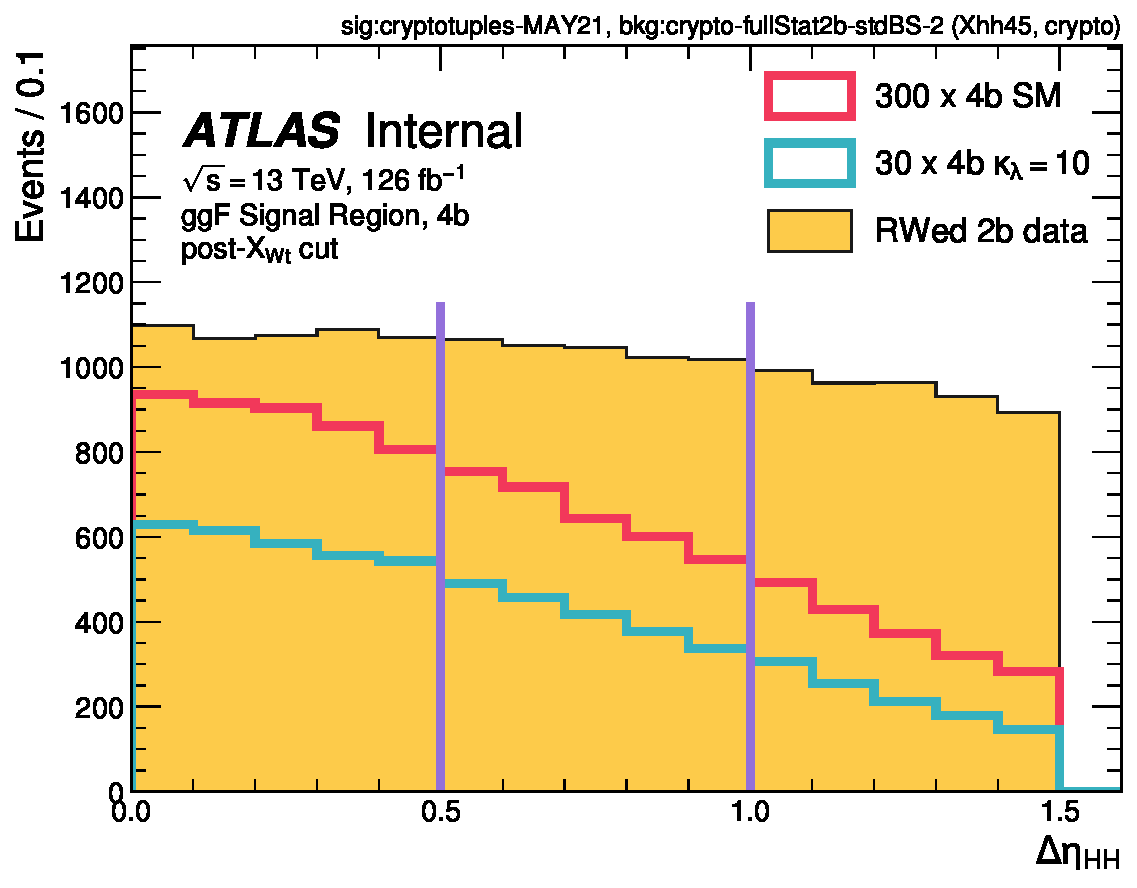
\includegraphics[width=0.4\textwidth]{figures/nr-int-note/category/V3/dEta_hh_sr_sig_bkg_4b_allyears}
	}
	\subfloat[All year merge: 4b ggF \Xhh]{ 
	    	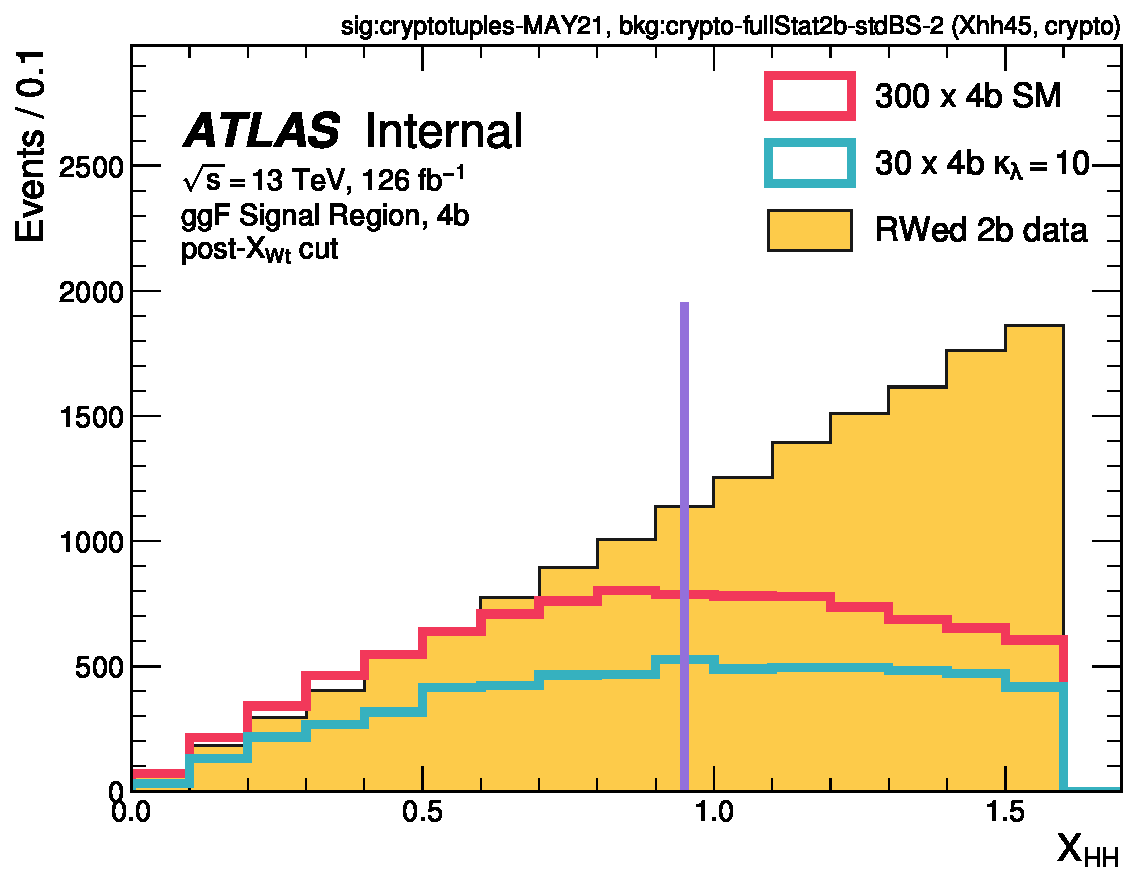
\includegraphics[width=0.4\textwidth]{figures/nr-int-note/category/V3/X_hh_sr_sig_bkg_4b_allyears}
	} 
	\caption{Distributions of the variables used for categorization in the ggF channel.
	Years are merged.
	To visualize the signals they are scaled by $\alpha = 100$ and 10 for the SM NR and $\kappa_\lambda$ = 10 signals, respectively.}
	\label{fig:ggF-4b-deta-xhh-SR}
\end{figure}

As discussed in \Sect{\ref{sec:bkgdestimation}}, the ggF background estimate is derived separately for the years, so we also fit the years separately as visualized in the 4b ggF histograms in \Fig{\ref{fig:ggF-4b-disc-log}}, with the SM and $\kappa_\lambda$ = 10 signals overlaid. The subpanels on these plots show the $S / \sqrt{B}$ significance to visualize which categories drive the sensitivity of the fit.
The signal peaks for the lower \deta, \Xhh values, so these are the higher purity categories that drive our significance.
The same plots with a linear y-axis are shown in \Fig{\ref{fig:ggF-4b-disc}}.

\begin{figure}[ht]
	\centering
	\subfloat[2016: 4b ggF]{ 
	    	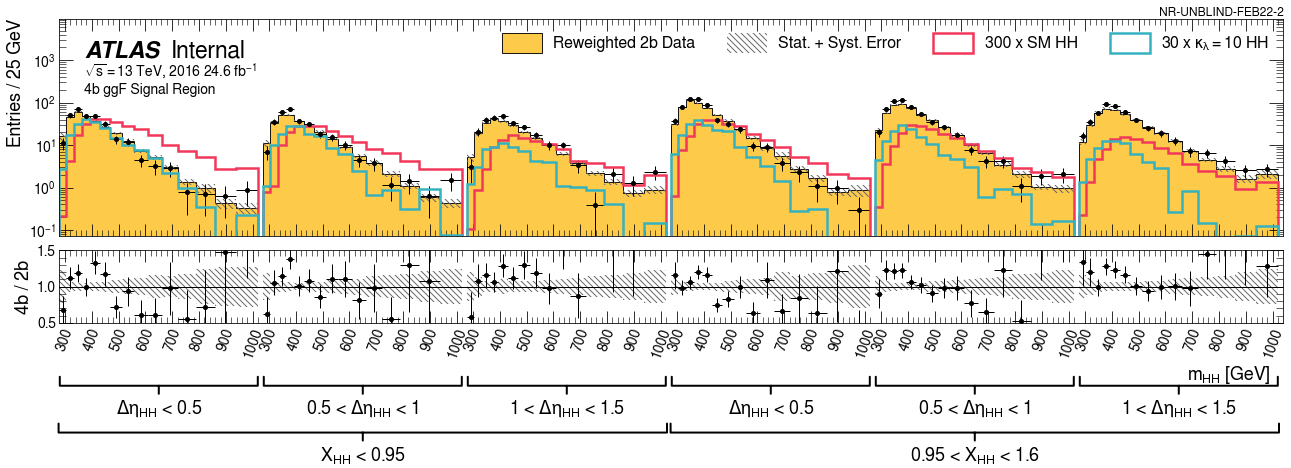
\includegraphics[width=\textwidth]{figures/nr-int-note/category/V4/m_hh_ggF_3_dEta_2_Xhh_ggF_16_4b_log.png}
		\label{fig:ggF-16-4b-log}
	} \\
	\subfloat[2017: 4b ggF]{ 
	    	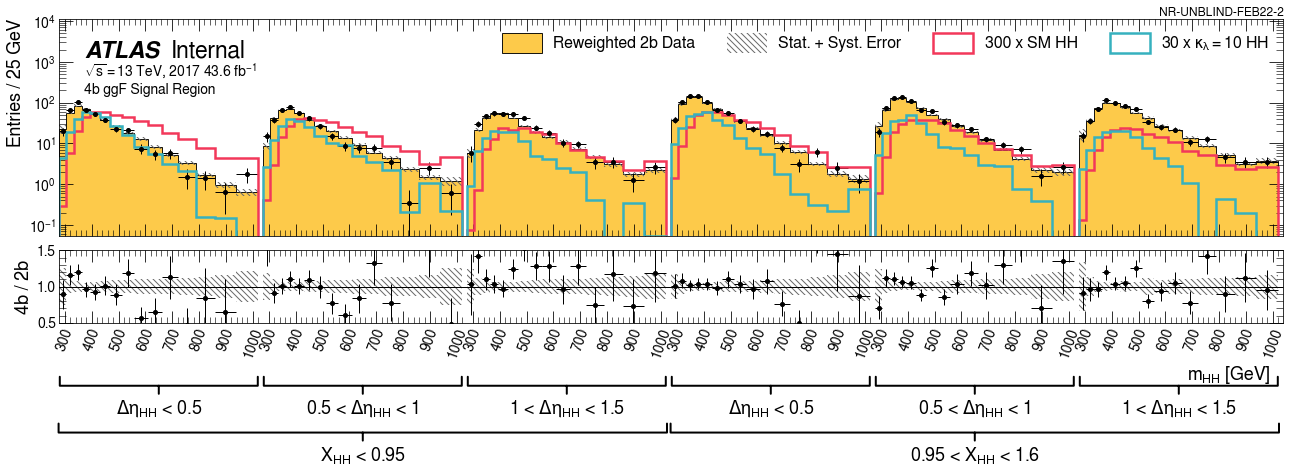
\includegraphics[width=\textwidth]{figures/nr-int-note/category/V4/m_hh_ggF_3_dEta_2_Xhh_ggF_17_4b_log.png}
		\label{fig:ggF-17-4b-log}
	} \\
	\subfloat[2018: 4b ggF]{ 
	    	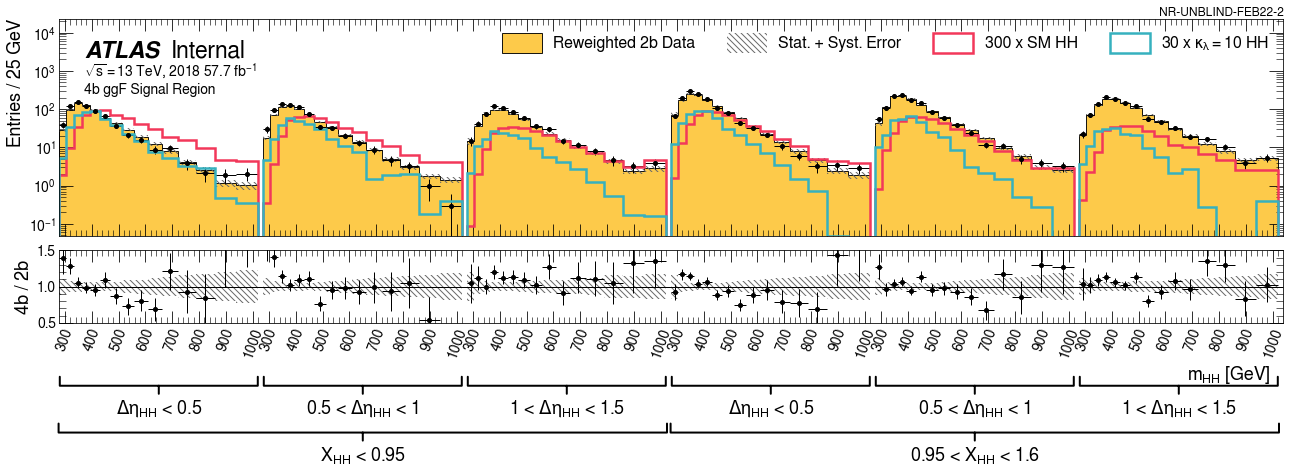
\includegraphics[width=\textwidth]{figures/nr-int-note/category/V4/m_hh_ggF_3_dEta_2_Xhh_ggF_18_4b_log.png}
 		\label{fig:ggF-18-4b-log}
	}
	\caption{4b \ ggF background and selected signal histograms for 2016, 2017, and 2018 with the proposed binning and categorization. To visualize the signals they are scaled by $\alpha = 100$ and 10 for the SM NR and $\kappa_\lambda$ = 10 signals, respectively.}
	\label{fig:ggF-4b-disc-log}
\end{figure}

\begin{figure}[ht]
	\centering
	\subfloat[2016: 4b ggF]{ 
	    	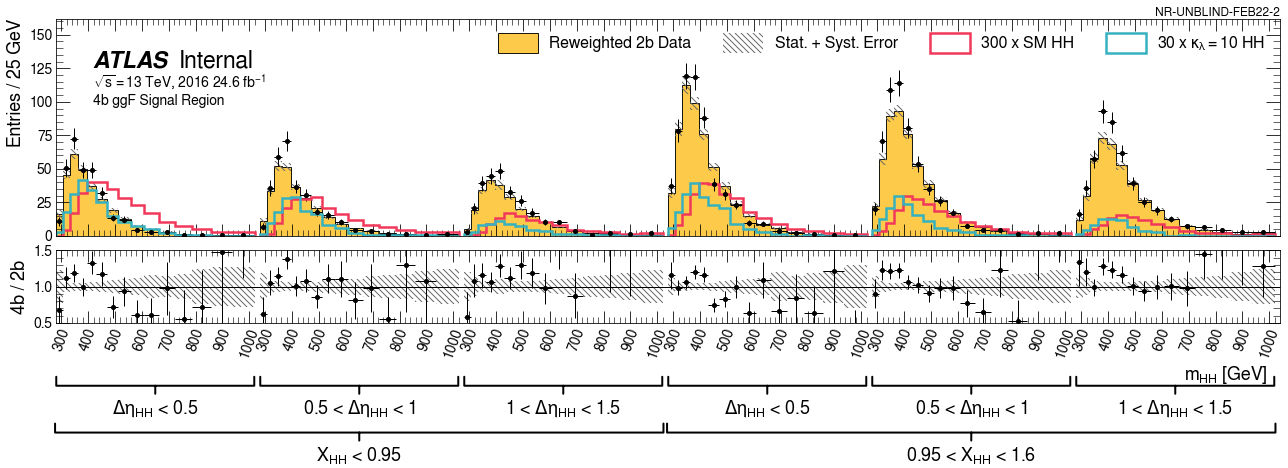
\includegraphics[width=\textwidth]{figures/nr-int-note/category/V4/m_hh_ggF_3_dEta_2_Xhh_ggF_16_4b.png}
		\label{fig:ggF-16-4b}
	} \\
	\subfloat[2017: 4b ggF]{ 
	    	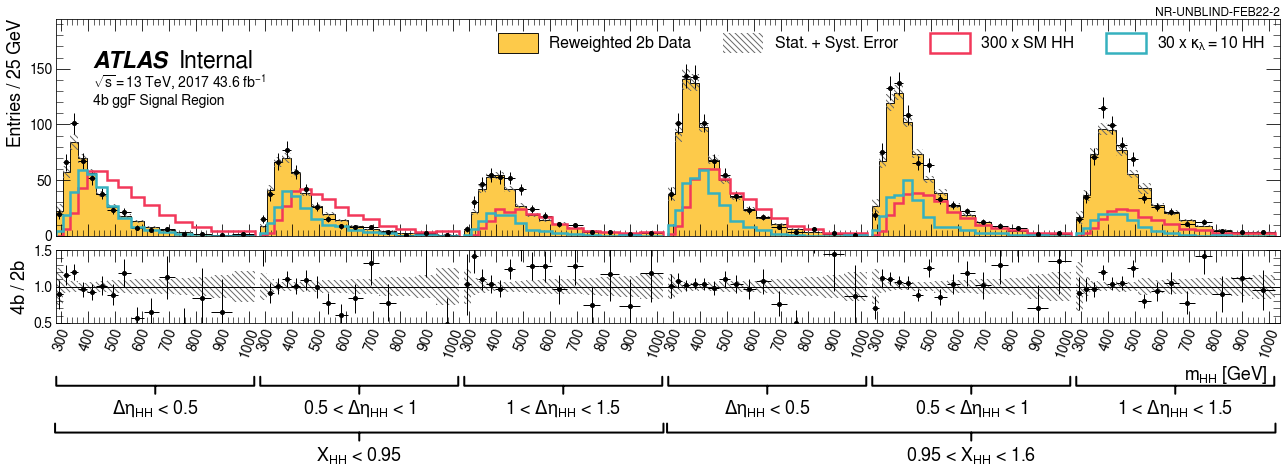
\includegraphics[width=\textwidth]{figures/nr-int-note/category/V4/m_hh_ggF_3_dEta_2_Xhh_ggF_17_4b.png}
		\label{fig:ggF-17-4b}
	} \\
	\subfloat[2018: 4b ggF]{ 
	    	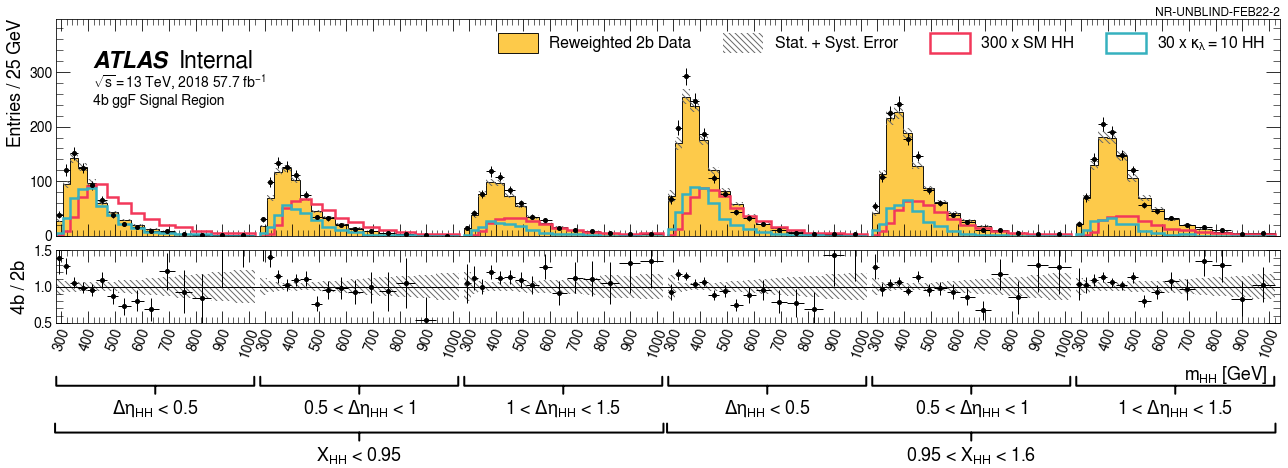
\includegraphics[width=\textwidth]{figures/nr-int-note/category/V4/m_hh_ggF_3_dEta_2_Xhh_ggF_18_4b.png}
 		\label{fig:ggF-18-4b}
	}
	\caption{4b \ ggF background and selected signal histograms for 2016, 2017, and 2018 with the proposed binning and categorization. To visualize the signals they are scaled by $\alpha = 100$ and 10 for the SM NR and $\kappa_\lambda$ = 10 signals, respectively.}
	\label{fig:ggF-4b-disc}
\end{figure}


%\Figure{\ref{fig:ggF-4b-disc-srs}} shows the histograms inclusive for the years, but separately visualizing the categories for the inside (\Xhh < 0.95) and outside (0.95 < \Xhh < 1.6) SRs.
% Visualizing the 4b discriminant separately as two SRs
% Commented out b/c non-trivial edits w/ our BS prescription
%\foreach \btag in {4b}{
%    \begin{figure}[ht]
%        	\centering
%        	\subfloat[2016--2018: \ \btag \ ggF SRin]{ 
%        	    	\includegraphics[width=\textwidth]{m_hh_ggF_3_dEta_2_Xhh_ggF_all_\btag_SRin.png}
%        	} \\
%        	\subfloat[2016--2018: \ \btag \ ggF SRout]{ 
%        	    	\includegraphics[width=\textwidth]{m_hh_ggF_3_dEta_2_Xhh_ggF_all_\btag_SRout.png}
%        	} \\
%        	\caption{\btag \ ggF background and selected signal histograms stacking the years (2016-2018) with the proposed binning and categorization. To visualize the signals they are scaled by $\alpha = 300$ and 10 for the SM NR and $\kappa_\lambda$ = 30 signals, respectively.}
%        	\label{fig:ggF-\btag-disc-srs}
%    \end{figure}
%}

\FloatBarrier
\clearpage

\subsubsection{VBF categories}
\label{subsubsec:VBF-cats}

%The VBF analysis has a single categorization based upon the pseudorapidity difference between the two reconstructed Higgs bosons, $\deta$.
The VBF analysis has a single categorization based on \deta.
The boundary for the categorization is 1.5, chosen as it satisfied the balance between maximizing significance and maintaining the accuracy of the modeling of the background within the categories.

Figure \ref{fig:vbf-detahh} shows the \deta distributions before and after the $X_{wt}$ cut for three key couplings -- $\kappa_{\lambda} = 10$, $\kappa_{2V} = 0$ and the Standard Model prediction -- alongside 4b data and the background estimate.

As shown in these plots, the $\deta$ distribution corresponding to the non-SM couplings peaks close to $\deta = 0$. On the other hand, the distribution corresponding to the SM prediction peaks at approximately \deta = 2. As such, the \deta < 1.5 category drives the sensitivity to the non-SM couplings; whereas, the $\deta \geq 1.5$ category is more sensitive to the SM prediction.

% SCRIPT: hh4b-plots/notebooks/Category-cut.ipynb
\begin{figure}[h]
	\centering
	\subfloat[Full mass plane with SR data blinded.]{ 
		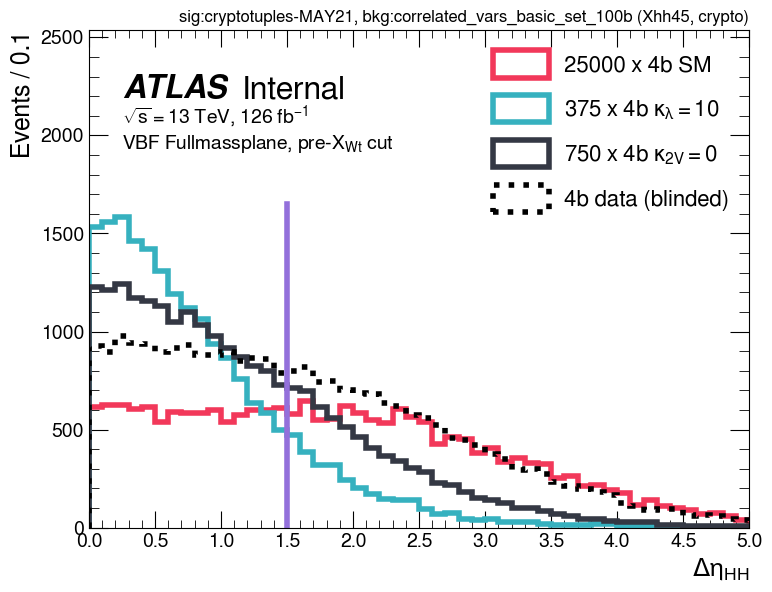
\includegraphics[width=0.45\textwidth]{figures/nr-int-note/category/V3/dEta_hh_VBF_fmp_sig_4bdata_allyears}
	\label{fig:vbf-detahh-4bdata}
	}
	\subfloat[SR with reweighted 2b background estimate.]{ 
		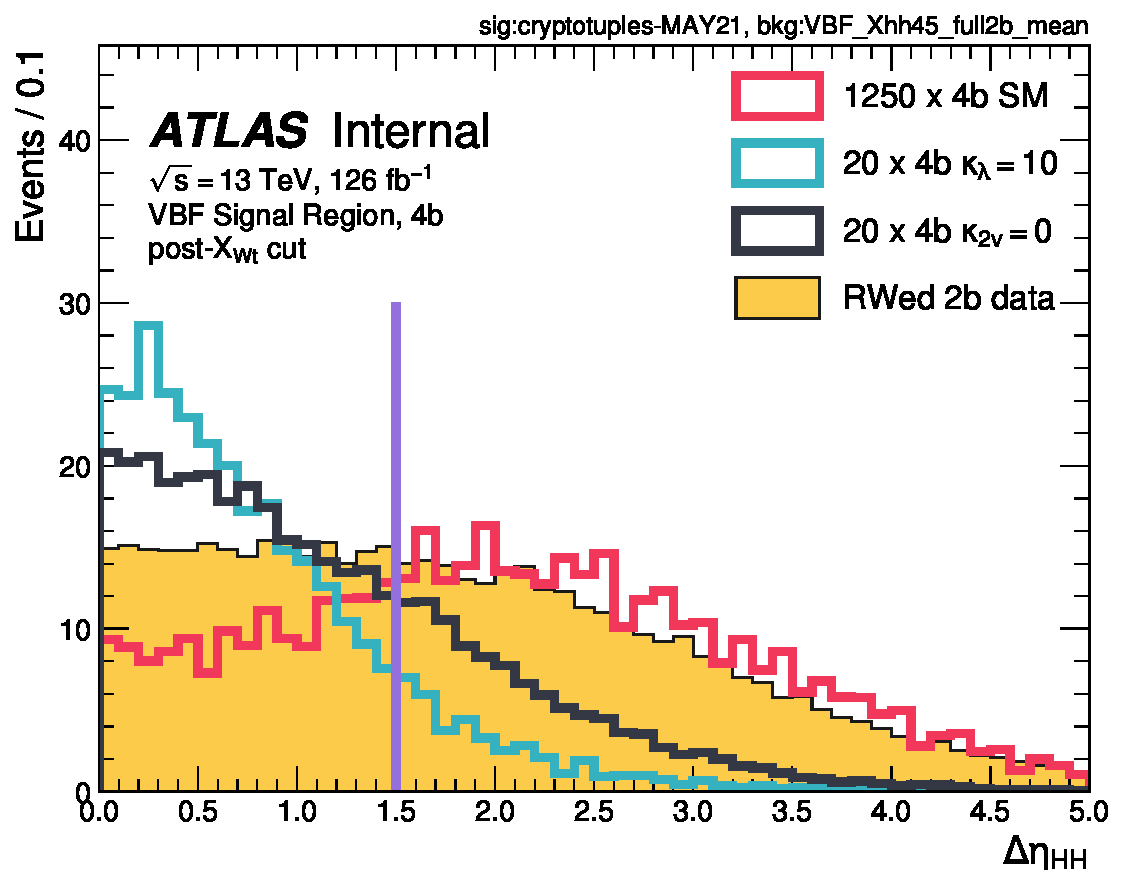
\includegraphics[width=0.45\textwidth]{figures/nr-int-note/category/V3/dEta_hh_VBF_sr_sig_bkg_allyears}
	\label{fig:vbf-detahh-bkg}
	}
	\caption{Distributions of the difference in pseudorapidity of the two reconstructed Higgs bosons ($\deta$) for signal Monte Carlo simulation, data and the background estimate in the VBF channel. The categorisation boundary is shown as a straight purple line at 1.5. The lefthand plot, Figure \ref{fig:vbf-detahh-4bdata}, shows the pre-$X_{wt}$ cut distributions for three key couplings -- $\kappa_{\lambda} = 10$, $\kappa_{2V} = 0$ and the Standard Model prediction -- alongside the 4b data distribution excluding events in the Signal Region. The righthand plot, Figure \ref{fig:vbf-detahh-bkg}, shows the post-$X_{wt}$ cut distributions for the same couplings alongside the reweighted 2b distribution that is used to estimate the background contribution. All signal distributions have been scaled up as to be visible next to data and reweighted data.}
	\label{fig:vbf-detahh}
\end{figure}

Figure \ref{fig:vbf-mhh-same} shows the reconstructed \HH mass distributions for the aforementioned three key couplings and the reweighted 2b data used to model the background contribution. Again, the signal distributions are scaled as to be visible next to the background estimate. Additionally, the significance of the scaled signal ($\alpha \times S/\sqrt{B}$) in each of the histogram bins is shown. The same signal scaling is used for each coupling across the two categories. This allows the sensitivity in the two categories to be compared. 

Due to the low significance below \SI{400}{\GeV} and poor modelling (\Fig{\ref{fig:Control-Region-1all-4b-8}}), we decided to drop the bins of \mhh < \SI{400}{\GeV} in the fit in both categories.

The significance of the $\kappa_{2V} = 0$ signal in the final bin in both plots in Figure \ref{fig:vbf-mhh-same} is far larger than in those preceeding it. The events in the overflow are placed in the final bin for visual purposes, and this is where the increase in signal, and therefore significance, originates. Separating the overflow into finer bins has the potential to improved results by accounting for information on the differing distribution shapes. However, this is a region low in data statistics, particularly 4b events. The binning used was optimized to account for as much shape information as possible whilst ensuring there were enough statistics in each bin for the asymptotic approximation, which is used to derive results, to hold. 

% SCRIPT: hh4b-plots/notebooks/Category-cut.ipynb

\begin{figure}[h!]
	\centering
	\subfloat[$\deta < 1.5$]{ 
		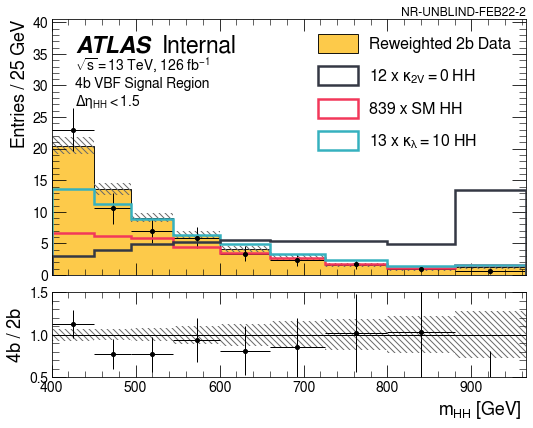
\includegraphics[width=0.45\textwidth]{figures/nr-int-note/category/V4/m_hh_VBF_2_dEta_all_4b_dEta_1.png}%{m_hh_VBF_2_dEta_VBF_all_4b_detahh_lt_1p5_same_scaling.png}
	\label{fig:vbf-mhh-lt-same}
	}
	\subfloat[$\deta \geq 1.5$]{ 
		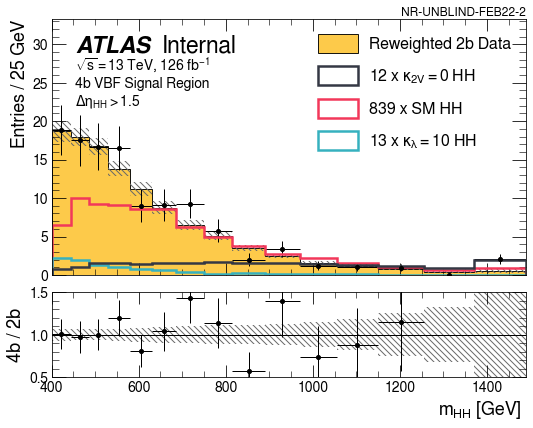
\includegraphics[width=0.45\textwidth]{figures/nr-int-note/category/V4/m_hh_VBF_2_dEta_all_4b_dEta_2.png}%{m_hh_VBF_2_dEta_VBF_all_4b_detahh_gt_1p5_same_scaling.png}
	\label{fig:vbf-mhh-gt-same}
	}
	\caption{Distributions of the reconstructed $m_{HH}$ for signal Monte Carlo simulation and the estimate of the background in each of the two $\deta$ categories in the VBF channel. Distributions for three of the key couplings are shown -- $\kappa_{\lambda} = 10$, $\kappa_{2V} = 0$ and the Standard Model prediction. Additionally, the significance of the scaled signal ($\alpha \times S/\sqrt{B}$) in each of the histogram bins is shown. Events in the underflow and overflow bins are counted in the yields of the initial and final bins respectively. The signals distributions are scaled as to be visible on the plot, and the scaling for each coupling is the same across the two categories.}
	\label{fig:vbf-mhh-same}
\end{figure}

\FloatBarrier
\clearpage

